\documentclass[a4paper,10pt]{scrartcl}
\usepackage{mathe-vorlesung}
\usepackage{graphicx}
\renewcommand{\equiv}{\Longleftrightarrow}
\newcommand{\eps}{\varepsilon}
\newcommand{\del}{\delta}
\newcommand{\homo}{\cong}
\renewcommand{\bigsqcap}{\prod}
\usepackage{txfonts}

\title{Topologie}

\begin{document}

\maketitle

\tableofcontents
\newpage
\begin{center}
\LARGE\textbf{Vorwort}
\end{center}
\begin{seg}{Was ist Topologie?}
\begin{itemize}
\item "` Unterzeichnung geometrischer Objekte bis auf stetige Dekorationen. "'
\item "` Stetigkeitsgeometrie"', "` qualitative Geometrie "', "`Gummi-Geometrie"'
\end{itemize}
Objekte werden in der Topologie als gleich angesehen, wenn sie durch eine in beiden Richtungen stetige bijektive Abbildung aufeinander abgebildet werden kann ("` Homöomorphismus"').
\end{seg}
So zum Beispiel für Teilmengen des $\R^2$:
\begin{figure}[h]
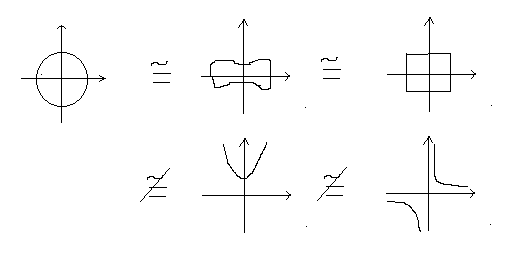
\includegraphics[scale=0.7]{fig1.png}
\end{figure}
\begin{ex*} 
Topologische Begriffe sind beispielsweise \emph{Stetigkeit, offene/abgeschlossene Mengen, Umgebung, Rand, Abschluss, Konvergenz, kompakt, zusammenhängend, Homotopie}.  Die konkreten Definition werden im Verlauf dieser Vorlesung geklärt.
\end{ex*}
\section{Grundbegriffe}
\subsection{Metrische und topologische Räume}
\begin{df}
Ein \emph{metrischer Raum} ist eine Menge $X$ zusammen mit einer Funktion $d: X \times X \rightarrow \R$, genannt Metrik oder \emph{Abstandsfunktion}, so dass folgende Axiome gelten:
\begin{enumerate}[\roman{enumi})]
\item \emph{Positivität}: $d(x,y)\ge 0 \land d(x,y)=0\equiv x=y$
\item \emph{Symmetrie}: $d(x,y)=d(y,x)$
\item \emph{Dreiecksungleichung}: $d(x,z) \le d(x,y)+d(y,z)$
\end{enumerate}
\end{df}
\begin{ex*}
Auf $\R^n$ ist durch die \emph{Euklidische Norm} $|x|=\sqrt{x_1^2+...+x_n^2}$ die \emph{Euklidische Abstandsfunktion} $d(x,y)=||x-y||$ gegeben. Auf $\R$ oder auf $\C$ ist diese Metrik durch den Betrag $d(x,y):=|x-y|$ definiert.  Man erhält auf diese Weise aus jeder Norm eine Metrik. Hierbei liefern verschiedene Normen natürlich verschiedene Metriken. Hier einige Beispiele auf $\R^2$:
\begin{itemize} 
\item euklidische Norm: $||x||_2=\sqrt{x_1^2+x_2^2}$
\item Maximumsnorm: $||x||_\infty := \max(|x_1|, |x_2|)$
\item $\Eins$-Norm $||x||_1 := |x_1|+|x_2|$
\end{itemize}
\end{ex*}

\begin{ex*}
Die diskrete Metrik definiert durch:
\[
d(x,y)=\begin{cases}
  0, & \text{falls} x=y \\ 1, & \text{falls} x\neq y
\end{cases}
\]
\end{ex*}

Es lassen sich zwei zentrale mathematische Begriffe mit HIlfe von Abstandsfunktionen definieren:
\begin{itemize}
\item Konvergenz von Folgen
\item Stetigkeit von Abbildungen
\end{itemize}

\begin{df}[Konvergenz im metrischen Räumen]
Sei $X$ ein metrischer Raum und $x_N, n\in \N$ eine Folge in $X$. Wir sagen $(x_n)_{n\in \N}$ \emph{konvergiert}, falls es ein $a \in X$ gibt, so dass gilt:
\[
\forall_{\varepsilon>0}\exists_{k\in\N}\forall_{n\ge k}: d(x_n,a)<\varepsilon
\]
\end{df}
In diesem Fall sagen wir, $a$ ist der \emph{Limes} (oder Grenzwert) von $(x_n)_{n\in \N}$ (und schreiben $x_n\rightarrow a, \lim\limits_{n\rightarrow \infty} x_n=a$) 

\begin{st} In einem metrischen Raum ist der Limes eine konvergente Folge eindeutig bestimmt.
\end{st}
\begin{proof}
Seien $a$ und $b$ Limiten von $(x_n)_{n\in \N}$ mit $\delta := d(a,b)>0$.

Da $(x_n)_{n\in \N}$ gegen $a$ konvergiert, gibt es $k\in \N$, sodass $d(x_n,a)<\frac{\delta}{2}$ für alle $n \ge k$.
Dann gilt nach Dreiecksungleichung:
\[
\delta=d(a,b)\le \underbrace{d(x,x_n)}_{<\frac{\delta}{2}}+d(x_n,b)
\]
Also gilt $d(x_n,b)\ge \frac{\delta}{2}$ für alle $n\ge b$, was der Konvergenz gegen $b$ widerspricht.
\end{proof}
\begin{df}[$\eps$-$\delta$-Definition der Stetigkeit in metrischen Räumen]
Seien $X$ und $\tilde X$ metrische Räume mit Abstandsfunktion $d$ bzw. $\tilde d$. Eine Abbildung $f: X \rightarrow \tilde X$ heißt stetig in$x \in X$ falls gilt: 
\[\forall_{\eps>0}\exists_{\delta>0} \forall_{x'\in X}: d(x,x')<\delta \implies \tilde d(f(x), f(x'))<\eps\]

Die Abbildung heißt \emph{stetig}, falls dies für alle $x\in X$ gilt.  Stetigkeit in metrischen Räumen hängen eng zusammen. Es gilt:
\end{df}
\begin{st}
Eine Abbildung $f: X\rightarrow \tilde X$ zwischen metrischen Räume ist genau dann stetig, wenn für jede konvergente Folge $x_n \rightarrow a$ in X gilt, dass $f(x_n) \rightarrow f(a)$
\end{st} 
\begin{proof}
\begin{seg}{"`$\implies$"'}
Sei $\eps>0$, dann gibt es $\delta>0$, so dass aus $d(x',a)<\delta$ folgt: $d(f(x'),f(a))<\eps$. Weiter gibt es ein $k\in \N$, so dass $d(x_N,a)y\delta$ für $n \ge k$.  Insgesamt folgt $d(f(x_n),f(a))<\eps$ für alle $n\ge k$.
\end{seg}
\begin{seg}{"`$\Longleftarrow$"'}
Angenommen, $f$ ist nicht stetig. Dann gibt es ein $x \in X$ und ein $\eps>0$, so dass es zu jeden $n\in \N$ ein $x$ mit $d(x_n,x)<\frac{1}{n}$ und $d(f(x_1), f(x))\ge \eps$ gibt. Damit ergibt sich der Widerspruch.
\end{seg}
\end{proof}
Die obigen Definition lassen sich mit Hilfe von $\eps$-Bällen umformulieren:
\begin{df}
Sei $X$ ein metrischer Raum und $x\in X$, dann heißt die Teilmenge 
\[
B_\eps(x)={x'\in X|d(x',x)<\eps}
\]
von $X$ heißt der (\emph{offene}) \emph{Ball mit Radius $\eps$ um x} (kurz: \emph{$\eps$-Ball}).
\end{df}
\begin{df}
In einem metrischen Raum heißt eine Teilmenge $U\subset X$ \emph{offen}, wenn es um jeden ihrer Punkte einen offenen $\eps$-Ball gibt, der ganz in U enthalten. Eine Teilmenge A heißt \emph{abgeschlossen}, wenn ihr Komplement $X\setminus A$ offen ist.  Eine Teilmenge $U \subset Y$ heißt \emph{Umgebung} eines Punktes $ x\in X$, falls es eine offene Teilmenge $V \subset X$ gibt mit $x\in v$ und $V \subset U$.  (Äquivalent: falls es ein $\eps$ mit $B_\eps(x)\subset U$ gibt.  
\end{df}

\begin{figure}[h]
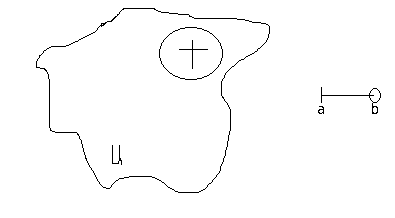
\includegraphics[scale=0.5]{fig3.png}
\end{figure}

Konvergenz und Stetigkeit lassen sich in metrischen Räumen durch offene Mengen beschreiben.
\begin{st}
In einem metrischen raum konvvergiert eine Folge $(x_n)_{n \in \N}$ genau dann gegen x, wenn es zu jeder Umgebung $U$ von $x$ ein $k \in \N$ gibt, so dass $x_n \in U$ für alle $n \ge k $ gilt.\\
\underline{Kurz:} Eine Folge $(x_n)_{n \in \N}$ konvergiert gegen $x$, wenn in jeder Umgebunng von $x$ \emph{fast alle} ($\hat =$ alle bis auf endlich viele) Folgenglieder liegen.
\end{st}
\begin{proof}
Die Äwuivalenz gilt, da jede Umgebung von $x$ einen $\eps$-Ball um $x$ enthält und umgekehrt jeden $\eps$-Ball um $x$ auch eine Umgebung von $x$ ist.
\end{proof}
\begin{st}\label{st:1.8}
Eine Abbildung zwischen metrischen Räumen $f: X\rightarrow \tilde X$ ist genau dann stetig in $x \in X$, wenn es zu jeder Umgebung $V$ von $f(X)$ eine Umgebung $U$ von $x$ gibt, so dass U unter $ f $ in V abgebildet wird; oder äquivalent dazu, falls das Urbild jeder Umgebung von $  f(x) $ eine Umgebung von x ist.
\end{st}
\begin{proof}
Dies folgt direkt aus der $ \eps $-$ \delta $-Definition der Stetigkeit und er Definition der Umgebung.
\begin{figure}[h]

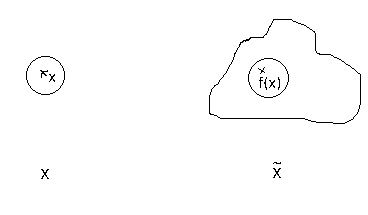
\includegraphics[scale=0.5]{fig4.png}
\end{figure}
\end{proof}
\begin{st}
Eine Abbildung zwischen metrischen Räumen ist stetig genau dann, wenn die Urbilder offener Mengen offen sind.
\end{st}
\begin{proof}
\begin{seg}{"`$\Longrightarrow$"'}
Sei $ f: X \to \tilde X $ stetig und $ V \subset \tilde Y $ offen.  Dann ist $ f^{-1}(V) $ nach \ref{st:1.8} eine Umgebung jeder ihrer Punkte somit offen.
\end{seg}
\begin{seg}{"`$\Longleftarrow$"'}
Seien umgekehrt die Urbilder offener Mengen offen und $ x \in X $. Sei $ \eps>0 $.  Nach Voraussetuuimg $ f^{-1}(B_\eps(f(x)) $ offen und enthält somit einen $ \delta $-Ball um den Punkt x.
\end{seg}
\end{proof}

Wichtige Beobachtung: Um Konvergenz und Stetigkeit zu beschreiben muss man nicht direkt auf eine Metrik Bezug nehmen, sondern es genügt das System der offenen Mengen zu kennen.  Dieses System von offenen Mengen nennt man \emph{die Topologie} des metrischen Raums .  Verschiedene Metriken können dieselbe Topologie erzeugen.

Alle Eigenschaften von metrischen Räumen, ihren Teilmengen oder Abbildung zwischen metrischen Räumen, die sich durch die Topologie (ohne direkten Bezug auf die metrik) beschreiben lassen, nennen wir \emph{topologische Eigenschaften}.

Dies führt zu dem folgenden Begriff:
\begin{df}
Sei $ X $ eine Menge und $O \in \mathcal P (x)$ eine Menge von Teilmengen von X; $ O $ heißt eine \emph{Topologie} auf $ X $, wenn folgendes gilt:
\begin{itemize}
\item[(T1)] Beliebige Vereinigungen von Mengen in $ O $ liegen wieder in O.
\item[(T2)] Die Schnittmenge von je zwei Mengen in $  O  $ liegt
\item[(T3)] Es gilt $ \emptyset \in O $ und $ X \in O$
\end{itemize}
Eine Menge $ X $ zusammen mit einer Topologie auf $ X $ heißt \emph{topologischer Raum}, die Elemente von $ O $ nennt man \emph{offene Teilmengen} von X, ihre Komplemente \emph{abgeschlossene Teilmengen}.
\end{df}
\begin{note*}
\begin{enumerate}[(\roman{enumi})]
\item Natürlich ist die Definition so gemacht, dass die in einem Topologie bilden. \fixme[fig5]
\item Verschiedene Metriken können diesselbe Topologie erzeugen, vgl. der aus der Analysis bekannter Satz, dass alle Normen auf dem $ \R^n $ äquivalent.  Daraus folgt: die Metrik die Metrik $ d(x,y) :=||x-y|| $ definiert für \emph{alle Normmen auf $ \R^n $} dieselbe Topologie, die sogenannte \emph{Standardtopologie}, zum Beispiel definieren:
\begin{align*}
d_1(x,y)&=|x_1-y_1|+...+|x_n-y_n|\\
d_2(x,y)&=\sqrt{(x_1-y_1)^2+...+(x_n-y_n)^2}\\
d_\infty(x,y)&=\max(|x_1-y_1|, ..., |x_n-y_n|)
\end{align*}
alle die Standardtopologie.
\end{enumerate}
\end{note*}
\begin{df}
Sei $ X $ ein topologischer Raum und  $x \in X $ Eine Teilmenge $ U \subset X $ heißt \emph{Umgebung} von x, wenn es eine offene Menge $ T\subset U $ gibt, die $ x $ enthält.  $ x $ heißt \emph{innerer Punkt} von A, wenn $ A $ eine Umgebung von $ x $ ist. $ x $ heißt \emph{äußerer Punkt}, falls $ X\setminus A $ eine Umgebung von x ist. Der Punkt $ x $ heißt Randpunkt von $ A $, falls keine von beiden gilt.  Die Menge $ \mathring{A} $ der inneren Punkte von $ A $ bezeichnet man als das \emph{Innere} von $ A $ oder als \emph{offener Kern} von $ A $. Die Menge $ \bar A $, der nichtäußeren Punkte von $ A $ heißt \emph{Abschluss} oder \emph{abgeschlossene Hülle} von $ A $.  Die Menge der Randpunkte von $  A $  heißt auch der Rand von A und wird mit $ \delta A $ bezeichnet. 
\end{df}

\begin{ex*}
Sei $ A=[a,b)\subset \R $ und sei $\R$ mit der Standardtopologie versuchen.  Dann gilt $\mathring A=(a,b), \bar A=[a,b], \delta A=\{a,b\}, B=\Q\subset \R$ gilt $ \mathring B=\emptyset, \bar B=\R, \delta B=\R $ 
\end{ex*}
\begin{ex}[Beispiele für Topologien]\label{thm:1.12}
\begin{enumerate}[(\roman{enumi})]
\item Durch Metriken definierte Topologie. Dies sind die sogenannten \emph{metrisierbaren Topologien}.
\item Die \emph{Klumpentopologie} $ O=\{\emptyset, X\} $ für eine beliebige Menge $ X $.  Sie ist nicht metrisierbar (falls $ X $ mehr als ein Element hat)
\item Die \emph{diskrete Topologie} $ O=\mathcal{P}(x) $ ist für jede beliebige Menge $ X $ definiert.  (Nur die schließlich konstanten Folgen sind konvergent.) Sie ist durch die diskrete Metrik gegeben.
\item Auf $\R^2$ ist durch
\[
O=\{A\subset \R^2|\forall_{(x,y)\subset A}\exists_{\eps>0}:(x-\eps,x+\eps) \times \{y\} \subset A\}
\]
eine Topologie gegeben. Übung: Ist diese metrisierbar?
\end{enumerate}

\end{ex}

\begin{df}
Sind auf einer Menge $X$ zwei Topologien $ O_1$ und $ O_2 $ gegeben, dann betrachten wir folgende Sprachweisen: gilt $ O_1 \subset O_2 $ , dann sagen wir $ O_2 $ ist \emph{feiner} als $ O_1 $ (und $ O_1 $ ist \emph{gröber} als $ O_2 $).  Gilt weder $ O_1 \subset O_2 $ noch $ O_2\subset O_1 $ , dann sagen wird, die Topologien $ O_1 $ und $ O_2 $ sind \emph{unvergleichbar}.
\end{df}

Auf jeder Menge ist die Klumpentopologie die größte mögliche Topologie und die diskrete Topologie, die feinst mögliche Topologie.  Die Topologie in \ref{thm:1.12}(iv) auf $ \R^2 $ ist feiner als die Standardtoplogie, aber gröber als die diskrete.

\begin{df}
Sei $ X $ ein topologischer Raum.  Eine Folge $ x_n $ heißt konvergent gegen $ a\in X $, falls jede Umgebung von $ a $ fast alle Folgenglieder enthält.
\end{df}
\begin{df}\label{thm:1.15}
Eine Abbildung $ f:X\to Y $ zwischen topologischen Räumen heißt \emph{stetig} in $ x\in X $, falls es zu jeder Umgebung $ V $ von $ f(x) $ eine Umgebung $ U $ von $ x $ gibt, so dass $ f(U)\subset V $ (Äquivalent: Falls das Urbild jeder Umgebung von $ x $ ist.) Die Abbildung heißt \emph{stetig}, wenn die Urbilder offener Mengen offen sind. Eine Abbildung zwischen topologischen Räumen, die bijektiv und stetig ist, heißt \emph{Homöomorphismus} (falls auch ihre Umkehrabbildung stetig ist.  Falls es einen Homöomorphismus $ d: X\to Y $ gibt, sagt man, $ X $ und $ Y $ sind \emph{homöomorph}, man schreibt: $ X\homo Y $.
Aus der Definition folgt sofort, dass eine Abbildung. $ f: X\to Y $ genau dann stetig ist, falls sie in jedem $ x\in X $ stetig ist. (zur Übung nachvollziehen)
\end{df}
\begin{st}
Sei $ f: X\to Y $ eine (in $ a\in X $) stetige Abbildung zwischen topologischen Räumen.  Sei $ x_n\to a $ konvergente Folge in $ X $. Dann gilt $ f(x_n) \to f(a) $
\end{st}
\begin{proof}
Sei $ V $ eine Umgebung von $ f(a) $. Da $ f $ (in $ a $) stetig ist, ist $ f^{-1}(V) $ eine Umgebung von $a$.  Wegen $ x_n\to a $ liegen fast alle $ x_n $ in $f^{-1}(V)$, somit gilt für fast alle $f(x_n)$ in $ V $.
\end{proof}
\begin{att}
Eine Abbildung, die jede konvergente Folge auf eine gegen das Bild des Limes konvergierende Folge abbildet (so eine Abbildung heißt \emph{folgenstetig}) ist \emph{im Allgemeinen nicht} notwendigerweise stetig. Siehe z. B. Joerich "`Topologie"' 6.3, bzw. später in der Vorlesung.
\end{att}
\begin{ex*}
\begin{enumerate}[(i)]
\item ist $ f: X\to Y $ eine stetige Abbildung und wird die Topologie auf X durch eine feinere oder die Topologie auf X durch eine gröbere ersetzt, bleibt $ f $ stetig.
\item Insbesondere ist \emph{jede} Abbildung $ f: X\to Y $ stetig falls $ Y $ die Klumpentopologie oder $ X $ die diskrete Topologie trägt.
\item In der Klumpentopologie ist \emph{jede} Folge gegen \emph{jeden Punkt} konvergent. 
\end{enumerate}
\end{ex*}
\begin{note}
Die Axiome eines topologischen Raums sind für sich alleine relativ schwach und lassen sehr viele Beispiele auch mit "`pathologischen"' Eigenschaften zu. Sie sind eher ein äußerer Begriffsrahmen. Um etwa Räume mit den von metrischen Räumen vertrauten Eigenschaften zu erhalten, muss man Zusatzannahmen machen.
\begin{itemize}
  \item "`Hausdorffeigenschaft"' $\implies$ Eindeutigkeit des Limes
  \item "`Abzählbarkeitsaxiome"' $\implies$ Äquivalenz von Stetigkeit und Folgendefinition
\end{itemize}
\end{note}
\subsection{Grundkonstruktionen}
Grundkonstruktionen sind Methoden, um neue Topologien zu definieren durch:
\begin{itemize}
\item Summe, teilräume, Produkte, Quotienten
\item durch Abbildungen zwischen topologischen Räumen
\end{itemize}
\begin{df}
Seien $ X $ und $ Y $ topologische Räume. Auf der disjunkten Vereinigung $ X \dot \cup V =X \times \{ 0 \} \cup Y \times \{1\}$ definieren wir eine Topologie durch:
\[
\{U \mathbin{\dot{\cup}} V| U \text{ offen in } X, V \text{ offen in } Y\}
\]
Der so entstehende topologische Raum $ X+Y $ wird als topologische Summe von X und Y bezeichnet (andere übliche Zeichen: $X \sqcup Y$ oder auch $X \perp Y$).
\end{df}
\begin{note*}
\begin{enumerate}[(i)]
\item Analog definert man die Summen von beliebig (auch unendlich) vieler topologischer Räumen $\biguplus_{\alpha \in  A} x_\alpha=\bigsqcup_{\alpha\in A} x_\alpha$, widerum als offene Menge $\{\dot \bigcup_{\alpha\in A}| U_\alpha \text{ offen in } X_\alpha \}$ setzt.
\item Für die disjunkte Verreinigung von Mengen $ X \dotcup Y $ ist auch die Schreibweise $X+Y:= X\times\{0\} \cup Y\times \{1\}$ üblich.  
\end{enumerate}
\end{note*}
\begin{ex*}
\begin{enumerate}[i]
\item Sei $ X=\{ x\} $ eine einelementige Menge. Dann ist die topologische Summe $ \biguplus_{\alpha\in A}X_\alpha $
\item Beispiel \ref{thm:1.12}(iv) ist homöomorph zu $ \biguplus_{\alpha\in \R} X_\alpha \R $ (Übung)
\end{enumerate}
\end{ex*}
\begin{df} Sei $ X $ ein topologischer Raum und $ M \subset X $. Die durch $ \{ U\cap M| U \text{ offen in } X \}$ auf $M$ defnierte Topologie heißt $ Teilraumtopologie $ (auch \emph{induzierte}, \emph{Relativ-} oder \emph{Spurtopologie}). 
\end{df}
\begin{ex*}
$X=\R^2, M=\{x-\text{Achse}\}$
\fixme{fig6}
\end{ex*}
\begin{att*}
Die offene Mengen $U\cap M$ in $ M $ sind im Allgemeinen nicht offen in $ X $ (es sei denn $ M\subset X $ wäre offen). Zum Beispiel:
\[
\text{T2: } (\underbrace{U_1}_{\text{offen in }X}\cap M)\cap (\underbrace{U_2}_{\text{offen in }X}\cap M)=(U_1\cap U_2)\cap M
\]
\end{att*}
\begin{df}
Seien $ X $ und $ Y $ topologische Räume. Eine Teilmenge $ W\subset X\times Y $ heißt offen bezüglich der Produktopologie auf $ X\times Y $ heißt offen bezüglich der Proudukttopologie auf $X\times Y$, falls es zu jedem Punkt $ (x,y)\in W $ eine Umgebung $ U $ von $ x $ und eine Umgebung $ V $ von $ y $ gibt, sodass $ U\times V $ in W enthalten ist.
\fixme{fig7}
\end{df}
\begin{note*}
\begin{enumerate}[(i)]
\item Die Standardtopologie auf $ \R^2 $ stimmt mit der Produkttopologie auf $ \R\times \R $ (beide Faktoren mit der Standardtopologie von $ \R $ versehen) überein.
\item Produkte offener Mengen in X und Y ("`Kästchen"') sind offen in den Produkttopoligien, aber nicht alle offenen Mengen sind Kästchen, z. B. sind auch die Vereinigung von Kästchen Kästchen.
\fixme{fig8} 
\end{enumerate}
\underline{Erinnerung:} Eine \emph{Äquivalenzrelation} auf einer Menge $ X $ ist eine Relation $\sim$ mit folgenden Eigenschaften:
\begin{enumerate}[(i)]
\item reflexiv: $a\sim a$
\item symmetrisch: $a\sim b \implies b\sim a$
\item transitiv: $a\sim b \land b \sim c\implies a\sim c$
\end{enumerate}
ist auf einer Menge $ X $ eine Äquivalenzrelation $\sim$ gegeben, so liegt jedes Element in seiner Äquivalenklasse
\[
 [x]:=\{y\in X|x\sim y\} \subset X
\]
und Äquivalenzklassen von zwei verschiedenen Elemente sind entweder disjunkt oder gleich; M zerfällt in die disjunkte Vereinigung der Äquivalenzklassen.  umgekehrt liefert eine Zerlegung einer Menge in disjunkte Teilmengen eine Äquivalenzrelation.
\end{note*}
\begin{df}
Sei X ein topologischer Raum und $\sim$ eine Äquivalenzrelation auf $ X $.  Sei $X/\sim$ die Menge der Äquivalenzklassen 
\[
X/\sim=\{[x]|x\in X\}
\]
und sei $ q: X\to X/\sim, x\mapsto [x] $ eine Teilmenge $ U $ von $ X/\sim $ ist genau dann offen bezüglich der \emph{Quotiententopologie} auf $ X/\sim $, wenn ihr Urbild $ q^{-1}(U) $ offen in X ist.
\end{df}

\begin{ex*}
\begin{enumerate}[(i)]
\item \begin{seg}{Zusammenschlagen eines Teilraums zu einem Punkt}
Sei $ X $ ein topologischer Raum und $ A\subset X $ ein Teilraum. Dann ist durch $ x \sim y :\equiv (x=y)\lor (x,y\in A) $ eine Äquivalenzrelation gegeben.  Zwei Punkte werden als äquivalent angesehen, wenn sie gleich sind oder beide in $ A $ liegen.
\end{seg}
\item \begin{seg}{Beispiel zu (i)}
Sei X ein topologischer Raum. Betrachte $ X\times [0,1] $
\fixme[fig9]
Man erhält den Kegel $CX:=X\times[0,1]/X\times\{1\}$
\end{seg}
\item Allgemeiner: "`\emph{Zusammenkleben}"'
\begin{enumerate}[(a)]
\item \fixme[fig10]
\item \fixme[fig11]
\end{enumerate}
bei (b) handelt es sich nicht um Zusammenschlagen eines Teilraums zu einem Punkt, sondern gegenüberliegend Punkte in den beiden senkrecht "`Radintervalle"' werden identifiziert mit den Äquivalenzrelationen: \fixme[nachschauen]
\[
(x_1,x_2)\sim (y_1,y_2):\equiv (x_1,x_2)=(y_1,y_2)\lor (x_1,y_1 \in \{0,1\} \land x_2 =y_2)
\]
\end{enumerate}
\end{ex*}
Eine weitere Möglichkeit aus gegebenen topologischen Räumen andere zu konstruieren, ist es, Topologien mit Hilfe von Abbildungen zu übertragen.
\begin{df}\label{thm:2.5}
\begin{enumerate}[(i)]
\item Sei $ X $ ein topologischer Raum und $ X $ eine Menge.  Sei $ f: X\to Y$ eine Abbildung.  Dann ist durch:
\[
\{U\subset Y|f^{-1}(U) \text{ offen} \}
\]
die \emph{finale Topologie} auf Y definiert.
\item Sei $ X $ eine Menge und $ X $ ein topologischer Raum.  Sei $ f: X\to Y $ eine Abbildung.  Dann ist durch 
\[
\{ f^{-1}(U)\subset X| U \text{ offen in } Y\}
\]
die \emph{initiale Topologie} auf X definiert.
\end{enumerate}
\end{df}
\begin{note*}
Die \emph{finale Topologie} ist die feinste Topologie auf Y die f stetig macht in (i). In (ii) ist die initiale Topologie die gröbste Topologie auf $ X $, die f stetig macht.
\end{note*}
\begin{exs*}
\begin{enumerate}[(i)]
\item Die Teilraumtopologie auf $M\subset X$ ist die initale Topologie bezüglich der \emph{Inklusionsabbildung} $ i:M\to X,m\mapsto m $, denn es gilt $ i^{-1}(U)=U\cap M $ für (offene) Mengen in $ X $.
\item Die Quotientenabbildung ist die finale Topologie bezüglich der Quotientenabbildung ist die finale Topologie bezüglich der Quotientenabbildung $ q: X\to X/\sim, x\mapsto [x] $
\item in ähnlicher Weise lässt sich die Summentopologie charakterisieren.  Sie ist die feinste Topologie, so dass beide Inklusionsabbildungen
$ i_X:X\to X+Y, x \mapsto x, i_Y: Y\to X+Y,y\mapsto y $ stetig sind.  Dies zeigt, dass es sinnvoll ist die Defnition \ref{thm:2.5} noch etwas weiter zu fassen.
\end{enumerate}
\end{exs*}
\begin{seg}{Zusatz zu Definition \ref{thm:2.5}}\label{thm:2.5(2)}
Allgemeiner definieren wir:
\begin{enumerate}[(i)]
\setcounter{enumi}{2}
\item Seien $X_i, i\in I$ topologische Räume und $ Y $ eine Menge. Sei durch $f_i:X_i\to Y, i\in I$ eine Familie von Abbildungen gegeben. Die feinste Topologie auf $ Y $, die alle Abbildungen $f_i$ stetig macht, heißt finale Topologie bezüglich $ f_i,i\in I $.
\[
\{U\subset Y|f^{-1}_i(U) \text{ offen in }X_i \text{ \emph{für alle}} i\in I\}
\]
$(T1) U_1, U_2\in O$ zeige: $U_1\cup U_2\in O$
\[f^{-1}(U_1\cup U_2)=\underbrace{f^{-1}_i(U_1)}_{\text{offen in } X_i}\cup \underbrace{f^{-1}_i(U_2)}_{\text{offen in } X_i}\]
\item Seien $ Y_i, i\in I $, topologische Räume und $ X $ eine Menge.  Seien $ f_i: X\to Y_i $ Abbildungen.  Die gröbste Topologie auf $ X $, die alle $f_i$ stetig macht, nämlich $\{f^{-1}_i\subset X| U \text{ offen in } Y, i\in I\}$ ist die \emph{initiale Topologie} bezüglich $f_i$. 
\end{enumerate}
\end{seg}
\begin{ex*}
Die Produkttopologie auf $ X\times Y $ ist initiale Topologie bezüglich der bei den kanonischen Projektionen
\[
\pi_X:X\times Y \to X, (x,y)\to x \text{ und } \pi_Y: X\times Y\to Y, (x,y)\to y 
\]
\end{ex*}
\begin{seg}{Erläuterung zu Definition \ref{thm:2.5} (iv)} 
Ist eine Familie $ S $ von offenen Teilmengen auf einer Menge $ X $ gegeben, so erhalten wir dadurch den \emph{Hüllenoperator} 
\[ 
\mathcal T(S):=\bigcap\limits_{ O \text{ Topologie auf } X \text{ mit } S\subset O} O 
\]
Die gröbste Topologie auf $ X $, die alle Mengen in $ S $ enthält. Die Topologie $ \mathcal T(S) $ nennt man auch die \emph{von $ S $ erzeugte Topologie} auf $ X $.
\end{seg}
Die in (iv) definierte Topologie ist also durch
\[
\mathcal T(\bigcup\limits_{i\in I} \{ f^{-1}(U)|U \text{ offen in } Y\} )
\]
\begin{ex*} Sei $ \R $ mit Standardtopologie versehen. Wir definieren eine Äquivalenzklasse $ [x] $ einer reellen Zahl $ x $ ist die Menge $x+\Z=\{x+k|k\in \Z\}$. Sei $ X=R/\sim $ mit der Quotiententopologie versehen. Wir \underline{behaupten}: $ X $ ist homöomorph zu $ Y:=\{v\in \R^2|\, ||v||=1\} $, den Einheitskreis in $ \R^2 $, mit der Teilraumtopologie versehen. \fixme[fig12]
\begin{proof}
Betrachte $ \phi(t)=(\cos(2\pi\cdot t),\sin(2\pi \cdot t)), \R\to Y $.
Wegen $ \phi(t+k)=\phi(t) $ für $ k\in \Z $, ist durch $ \bar\phi: X\to Y, [x]\to \phi(x) $ eine wohldefinierte Abbildung gegeben. $\bar \phi$ ist offensichtlich bijektiv. Die Abbildung $ \bar \phi  $ ist stetig nach Definition der Quotientenabbildung, da $ \phi $ stetig ist.

Es bleibt noch zu zeigen: Die Bilder offener Mengen sind offen (man sagt dann: $ \bar \phi $ ist \emph{offen}, dass heißt die Bilder offener nicht offen), dass heißt $ \bar \phi^{-1} $ ist stetig. Wir zeigen: Die Bilder bageschlossenen Mengen sind abgeschlossen: Sei $ A\subset X $ abgeschlossen. Dann ist $ q^{-1}(A)\subset \R $ abgeschlossen (mit $ q: \R\backslash \R/\sim $ die Quotientenabbildung).

Es gilt $ \bar \phi(A)=\phi(q^{-1}(A))=\phi(q^{-1}(A)\cap[0,1]) $. Da $ q^{-1}(A)\cap [0,1] $ kompakte Tielmenge von $C$ $ \R $ ist, ist $ \bar\phi(A)=\phi(\phi-1)(A)\cap[0,1]) $ kompakt, also abgeschlossene Teilmenge des $ \R^2  $ und somit von $ Y $.
\end{proof}
\end{ex*}
\subsection{Hausdorffräume}
\begin{df}[Hausdorffsches Trennungsaxiom]
 Ein topologischer Raum heißt \emph{Hausdorffraum}, wenn man zu je zwei verschiedenen Punkten disjunkte Umgebungen finden kann.
\\ \fixme[fig13]
\end{df}
\begin{st}
Jeder metrische Raum ist ein Hausdorffraum. 
\end{st}
\begin{proof}
Dies folgt aus der Dreiecksungleichung der Metrik. \\
 \fixme[fig14] \\
Seien $x$ und $y$ Punkte im metrischen Raum und sei $d(x,y)>0$.
Dann sind die beiden $\eps$-Bälle $B_\eps(x)$ und $B_\eps(y)$ mit $\eps:=\frac{1}{2}d(x,y)$ disjunkte Umgebungen von $x$ bzw. $y$. Dann 
wäre $z\in B_\eps \land B_\eps(y)$, dann wäre die Dreiecksungleichung
\[
\underbrace{d(x,z)}_{y<\eps}+\underbrace{d(z,y)}_{<\eps}\ge d(x,y)=2\eps
\]        
verletzt.
\end{proof}
\begin{st}
Jeder Teilraum eines Hausdorffraums ist Hausdorffsch. Zwei topologische Räume sind genau dann Hausdorffsch, wenn ihre topologische Summe es ist und zwei nichtleere topologische Räume sind Hausdorffsch, genau dann wenn ihr Produkt es ist. 
\end{st}
\begin{proof}[zur Übung]\end{proof}
\fixme[fig15]\\
Ein Raum, der nicht Hausdorffsch ist, scheint mit unserer Intuition unvereinbar zu sein.  Ein finales Beispiel ist die Klumpentopologie $\{\emptyset, X\}$ auf jeder Menge. Mit Hilfe der Quotiententopologie erhält man weniger triviale Beispiele von Nicht-Hausdorffräumen.
\begin{ex*} Für Nicht-Hausdorffraum:\\
Die Gerade mit einem Dppelpunkt. Sei $ X=\R+\R=\R\times \{0\}\cup \R\times \{1\} $. Definiere man $ (x,n)\sim (y,m)\stackrel{\text{def}}{\iff} x=y\neq 0 $. \\
\fixme[fig16]\\
$ \R $ besitzt unter Betrachtung dieser Relation doppelt vorhandene Nullpunkte.

Die beiden Punkte $(0,0)$ und $(0,1)$ in $ X/\sim $ lassen sich nicht durch disjunkte Umgebung trennen.\\
\fixme[fig17]\\
Wir wollen noch zwei weitere Eigenschaften von Hausdorffräumen beweisen, die mit der geometrischen Intuition übereinstimmen.
\end{ex*}
\begin{st}
In einem Hausdorffraum ist gilt:
\begin{enumerate}[(i)]
\item Der Limes einer konvergenten Folge ist eindeutig bestimmt.
\item Punkte sind abgeschlossen.
\end{enumerate}
\end{st}
\begin{proof}
\begin{enumerate}[(i)]
\item Seien $ a\neq b $ verschiedene Limiten einer konvergenten Folge $ x_n $, dann gibt es disjunkte Umgebungen $ U_a $ und $ U_b $ von $ a $ bzw. $ b $.  Da $ x_n $ gegen $ a $ konvergiert, liegen fast alle Folgenglieder in $ U_a $, im Widerspruch zur Konvergenz von $ x_n $ gegen $ b $.
\item Das Komplement einer einelementigen Menge ist offen, denn nach der Hausdorffeigenschaft gibt es um jeden ihrer Punkte eine Umgebung, die insbesondere p nicht enthält.
\end{enumerate}
\end{proof}
\fixme[fig18]
\begin{note*}
Dies liefert eine notwendige Bedingung dafür, dass eine QUotiententopologie Hausdorffsch ist.  Alle Äquivalenzklassen müssen abgeschlossen sein.
\end{note*}
\subsection{Zusammenhang und Wegzusammenhang}
\begin{df}
Ein topologischer Raum heißt \emph{zusammmenhängend}, wenn er sich nicht in zwei nichtleere, offene, disjunkte Teilmengen zerlegen lässt.
\end{df}
\fixme[fig19]
\begin{note*}
Äquivalent zu "`zusammenhängend"' sind:
\begin{enumerate}[(i)]
\item Die leere Menge und der ganze raum sind die einzigen Mengen, die sowohl offen als auch abgeschlossen sind.
\item Der Raum ist nicht homöomorph zu einer topologischen SUmme zweier nichtleere topologischer Räume.
\end{enumerate}
\end{note*}
\begin{exs*}
\begin{enumerate}[(i)]
\item Die leere Menge und der ganze Raum sind die einzigen Mengen, die sowohl offen als auch abgeschlossen sind.
\item Der Raum ist nicht homöomorph zu einer topologischen Summe zweier nichtleere topologischen Räume.
\item Ein Intervall $ I $ ist zusammenhängend: 
\begin{proof}
Angenommen $I=A\dotcup B$, beide $ A $ und $ B $ offen und abgeschlossen (in der Teilraumtopologie, durch $ I\subset \R $ induziert) Seien $ a\in A, b\in B $, wobei $ a<b $ ohne Einschränkung. Defniere $ s:=\inf\{x\in B|a<x\}$. Dann liegt in jeder Umgebung von $ s $ ein Punkt aus $ B $. (nach Definition des Infinums). Es gilt entweder $ s=a $ oder $ s>a $. Im ersten Fall kann $ s $ kein innerer Punkt von $ A $ sein, im zweiten Fall liegt das Intervall $ (a,s) $ ganz in $ A $ und $ s $ kann weder von $ A $ noch von $ B $ ein innerer Punkt sein. Dies führt letztlich zum Widerspruch.
\end{proof}
\end{enumerate}
\end{exs*}
Ein stärkerer Begriff ist der des \emph{Wegzusammenhangs} (Ein \emph{Weg} in einem topologischen Raum $ X $ ist eine stetige Abbildung $ [a,b]\to X $
\begin{df}
Ein topologischer Raum heißt \emph{wegzusammenhängend}, wenn es zu je zwei Punkte $ p,q\in X $ einen Weg gibt, dass heißt eine stetige Abbildung $ c: [0,1]\to X $ mit $c(0)=p, c(1)=q$.
\end{df}
\begin{ex*}
$ \R^n $ ist wegzusammenhängen, in der Tat, benutze man zum Beispiel $ c(t)=(1-t)p+tq $. \fixme[fig20]
\end{ex*}
\begin{st}
Ein wegzusammenhängender topologischer Raum ist zusammenhängend.
\end{st}
\begin{proof}
Angenommen $ X=A\dotcup B $, wobei $ A $ und $ B $ beide offen und nichtleer.  Sei $ p\in A $ und $ q\in B $ und $ c $ ein Weg zwischen p und q. \\ \fixme[fig21]\\
Dann wäre $[0,1]=c^{-1}(A)\dotcup c^{-1}(B)$ eine Zerlegung in zwei disjunkte, nichtleere offene Mengen.
\end{proof}
Die Umkehrung gilt jedoch im Allgemeinen nicht:
\begin{ex*}
Ein Raum, der zusammenhängend, aber nicht \underline{weg}zusammenhängend ist.
\[
X=\underbrace{\{0\}\times [-1,1]}_{A}\cup\underbrace{\{(x, \sin(x^{-1})|x>0\}}_{B}
\] 
\fixme[fig22]
\end{ex*}
Die Relation $ p\sim q \stackrel{\text{def}}{\iff} $ es gibt einen weg von $ p $ nach $ q $ ist (Übung) offensichtlich eine Äquivalenzrelation, die zugehörigen Äquivalenzklassen heißen \emph{Wegzusammenhangskomponenten} des topologischen Raums.
\begin{st}
\begin{enumerate}[(i)]
\item Stetige Bilder von (weg-)zusammenhängenden Räumen sind (weg-)zusammenhängend.
\item Vereinigungen (weg-)zusammenhängender Räume $ X_i, i\in I, $ mit $ \bigcap X_i\neq \emptyset $ sind wegzusammenhängend.
\item Ein Produkt $ X\times Y $ von (weg-)zusammenhängenden nichtleeren topologischen Räumen $ X,Y $ ist genau dann (weg-)zusammenhängend, wenn die beiden Faktoren es sind. 
\end{enumerate}
\end{st}
\begin{proof}
\item Sei $ f:X\to $ stetige Abbildung, so zerfällt $f(X)=Y_1\dotcup Y_2$ mit $Y_1, Y_2$ offen disjunkt, dann auch $ X=f^{-1}(Y_1)\dotcup f^{-1}(Y_2) $. \\
\fixme[fig23]
Sei $ p,q \in f(X) $. Es gibt $ a,b\in X $ mit $ f(a)=p $, $ f(b)=q $ und einen Weg $ c:[0,1]\to X $ von $ a $ nach $ b $. Dann ist $ f\circ c:[0,1]\to X $ ein Weg von $ p $ nach $ q $.
\item Sei $ X=\bigcup_{i\in I}X_i $. Sei $ X=A\dotcup B $ mit $ A,B $ offen. Sei $ p\in \bigcap_{i\in I}X_i $ und ohne Einschränkung $ p\in A $.  Es gilt $ X_i=(X_i\cap A)\dotcup (X_i\cap B) $, da $ p\in X_i\cap A $ folgt $ X_i\cap B=\emptyset $, denn $ X_i $ ist zusammenhängend. Also folgt $ B=\emptyset $.
Für Wegzusammenhängend:
\fixme[fig24]
Es gilt, falls $ c:[0,1]\to X_I $ estetiger Weg von $ a\in X_i $ nach $ p $ und $ d:[0,1]\to X_j $ stetiger Weg von $ p $ nach $ b\in X_j $, dann ist:
\[
e/t(:=\begin{cases}c(2t)\qquad &,t\in[0,\frac 1 2]\\ d(2t-1)\qquad &,t\in[\frac 1 2, 1]\end{cases}
\]
eine stetige Abbildung $ [0,1]\to \bigcup_{i\in I}X_i $. (Übung)
\end{proof}
\begin{df}
 Eine \emph{Zusammenhangskomponente} $e$ eines topologischen Raumes $X$ ist ein maximal zusammenhängender Teilraum.
($A\subset X$ ist \emph{maximal zusammenhängend}, falls es keine zusammenhängende Teilmenge $B\subset X$ gibt mit $A\subset B, A\neq B$)
\end{df}
\begin{st}\label{thm:4.4}
 \begin{enumerate}[(i)]
  \item Ist $A\subset X$ zusammenhängend und $A\subset B\subset \bar A$, so ist auch $B$ zusammenhängend.
  \item Jeder Punkt von $X$ liegt in genau einer Zusammenghangskomponente von $X$, mit anderen Worten. $X$ ist die disjunkte Vereinigung seiner Komponenten.
\item Die Komponenten von $X$ sind abgeschlossene Teilräume.
 \end{enumerate}

\end{st}

\begin{proof}
 \begin{enumerate}[(i)]
  \item Seien $M_1,M_2\subset X$ abgeschlossen mit $B\subset M_1\cup M_2$ und $B\cap M_1\cap M_2=\emptyset$. 
Sei ohne Einschränkung $A\cap M_1\neq$. Zu zeigen ist, dass $B\cap M_2=\emptyset$. Da $A$ zusammenhängend ist, gilt $A\subset M_1$, also auch $\bar A \subset M_1$, somit gilt $B\cap M_2=\emptyset$.
\item Die Vereinigung aller zusammenhängenden Teilräume von $X$, die den Punkt $p$ enthalten, ist nach \ref{thm:4.4}(ii)
 zusammenhängend und offenbar die einzige maximal zusammenhängende Teilmenge, die $p$ enthält. (Immer ist $\{p\}$ zusammenhängend)
\item folgt aus (i).
 \end{enumerate}
\end{proof}
\subsection{Abzählbarkeitsaxiome}
\begin{df}
 Sei $(X,O)$ ein topologischer Raum. Eine Teilmenge $\mathcal B\subset O$ heißt \emph{Basis}(die Topologie) von $X$, wenn jedes $U\subset O$ eine Vereinigung von Mengen aus $\mathcal B$ ist.
\end{df}
\begin{exs*}
 \begin{enumerate}
  \item Immer gilt, dass $O$ selbst eine Basis ist.
  \item Im $\R^n$ ist der Menge der offenen $\eps$-Bälle eine Basis der Topologie, aber auch die Menge der achsenparallelen offenen Würfel.
  \item Allgemeiner ist in jedem metrischen Raum die Menge der offenen $\eps$-Bälle eine Basis der Topologie.
  \item Seien $(X_1,O_2)$ und $(X_2,O_2)$ topologische Räume. Dann ist $O_1\times O_2$ eine Basis der Produkttopologie.
\end{enumerate}
\end{exs*}
Kann man beliebige Familien von Teilmengen eines Raumes $X$ vorgeben und fordern, die Topologie solle aus allen Vereinigungen dieser Mengen (und $X$ selbst) bestehen? Nein, man muss auch sicherstellen, dass endliche Schnitte wieder offen sind. Deshalb:
\begin{df}
 Sei $(X,O)$ ein topologischer Raum. Eine Teilmenge $\mathcal S\subset O$ heißt \emph{Subbasis}, wenn die Menge der endlichen Schnitte der Mengen in $\mathcal S$ eine Basis bildet.
\end{df}
\begin{st}\label{thm:4.3}
 Sei $X$ eine Menge und $\mathcal S\subset \Pot(X)$  eine Familie von Teilmengen von $X$. Dann gibt es genau eine Topologie auf $X$, die dieses $S$ als Subbasis hat.
\end{st}
\begin{proof}
Sei $\mathcal B:=\{\S_1\cap...\cap S_n|n\in \N_0, S_1,...,S_n\in \mathcal S\}$ und setze $O:=\{\bigcup_iB_i|i\in \mathcal B\} \cup\{\emptyset,X\}$.
 Wir zeigen, dass $O$ eine Topologie auf $X$ ist. Offensichtlich liegen beliebigen Vereinigung von Mengen in $O$ wieder in $O$. 
Sei $U_1=\bigcup_{i\in I_1}B_i, U_2=\bigcup_{i\in I_2}B_i$, mit $B_i\in \mathcal B$. Dann ist:
\[
 U_1\cap U_2=\bigcup\limits_{j\in I_1,k\in I_2}B_j\cap B_k
\]
eine Vereinigung von endlichen Schritten von Mengen in $\mathcal S$, also Element von $O$. (Dies zeigt, dass $O$ eine Topologie auf $X$ ist). 
Jede Topologie auf $X$, die $\mathcal S$ enthält, muss auch $O$ enthalten, anderer seits kam eine Topologie mit $\mathcal S$ als Subbasis auch nicht feiner sei als $O$.
\end{proof}
Man sagt auch, $O$ ist die \emph{von $\mathcal S$ erzeugte Topologie}. Dass heißt $O$ entsteht durch Anwenden des früher definierten
Hüllenoperators auf $\mathcal S$, $\mathcal T(\mathcal S)=\emptyset$.

Als eine Anwendung wollen wir die Produkttopologie von beliebig (auch unendlich) vielen Räumen erklären.

Seien $(X_\alpha,O_\alpha), \alpha A$ topologische Räume und sei
\[
 \bigsqcap X_\alpha=\{f:A\to\bigcup X_\alpha|f(\alpha)\in X_\alpha\}
\]
Wir verwenden als Subbasis die Menge
\[
 \mathcal S:=\{\bigsqcap_\alpha U_\alpha\in O_\alpha, U_\alpha=X_\alpha \text{ für alle bis auf ein $\alpha \in A$}\}
\]
Die so (nach Satz \ref{thm:4.3}) defnierte Topologie heißt \emph{Produkttopologie} auf $\bigsqcap_\alpha X_\alpha$ (und 
$\mathcal S$ ist eine Subbasis). Dann ist:
\[
 \mathcal B := \{ \bigsqcap_\alpha U_\alpha|U_\alpha\in O_\alpha, U_\alpha=X_\alpha \text{ für alle bis auf endlich viele } \alpha \in A\}
\]
\begin{seg}{Übungsaufgabe}
 Nach Konstruktion ist die Produkttopologie die initiale Topologie bezüglich der kanonischen Projektionen $\pi_\alpha:\bigsqcap_\alpha X_\alpha\to X_\alpha: f\mapsto f(\alpha)$
Die kanonische Projektionenen sind nämlich stetig: Sei $\alpha \in A$. Das Urbild $\pi_\alpha^{-1}$ einer offenen Menge $U\subset X_\alpha$ ist gerade:
\[
 \{\bigsqcap_\beta U_\beta|U_\alpha=U, U_\beta=X_\beta \text{ für } \beta\neq a\}
\]

\end{seg}
\begin{note*}
 \begin{itemize}
  \item $\mathcal S=(X_1,X_2,...,X_{k-1}, U, X_{k+1},...,X_n$ mit $U\subset X_k$ offen,$A={1,...,n}$
  \item $\R^3=\{(x_1,x_2,x_3)|x_\alpha\in \R\}$, $\R^3=\{f:\{1,2,3\}\mapsto \R, \alpha\mapsto x_\alpha\}$
 \end{itemize}
\end{note*}
\begin{df}
 Sei $(X,O)$ ein topologischer Raum. Eine Familie $\mathcal U$ von Umgebungen von $p$ heißt \emph{Umgebungsbasis} von $p$, wenn jede Umgebung von $p$ eine Umgebung aus U enthält.
\fixme[fig25]
\end{df}
\begin{exs*}
 \begin{enumerate}
\item  Im $\R^n$ ist zum Beispiel ist $
 \{B_\eps(p)|\eps>0\}$ eine Umgebungsbasis von $p$, aber auch $ \{B_\eps(p)|\eps\in (0,1]\}$ und $\{ B_\eps(p)|\eps>0,\eps\in \Q \}$ die letzte ist abzählbar auch $\{B_{n^{-1}}(p)|n\in \N\}$
\item Dies lässt sich auf metrische Räume übertragen: In jedem metrischen Raum $X$ mit $p\in X$ ist $\{B_{n^{-1}}(p)|n\in \N\}$ eine abzählbare Umgebungsbasis von p.
 \end{enumerate}
\begin{df}
 \begin{enumerate}[(i)]
  \item Ein topologischer Raum erfüllt das \emph{erste Abzählbarkeitsaxiome}, wenn es um jeden Punkt eine abzählbare Umgebungsbasis gibt. 
\item Ein topologischer Raum erfüllt das \emph{zweite Abzählbarkeitsaxiome}, wenn es eine abzählbare Basis der Topologie gibt.
 \end{enumerate}

\end{df}
\end{exs*}
\begin{seg}{Zusammenfassung}
\begin{itemize}
 \item \emph{Basis}, wenn sich jede offene Teilmengen als Vereinigung dieser Menge bilden lässt.
 \item \emph{Subbasis}, wenn endliche Schnitte eine Basis bilden.
 \item \emph{Abzählbarkeitsaxiome}
 \begin{itemize}
\item \emph{Erstes Abzählbarkeitsaxiom}: Um jeden Punkt gibt es ein abzählbare \emph{Umgebungsbasis}(Umgebungsbasis von $p\in X$: eine Familie von Teilmengen $U$
, wenn jede Umgebung von p eine Menge aus $U$ enthält.)
\item \emph{Zweites Abzählbarkeitsaxiom}: Der Raum besitzt eine abzählbare Basis
\end{itemize}
\end{itemize}
\end{seg}
Der folgende Satz gibt eine Antwort auf die Frage, wie die beiden Abzählbarkeitsaxiome zusammenhängen und eine Antwort auf die Frage, wozu das erste Abzählbarkeitsaxiom nützlich ist.
\begin{st}
 \begin{enumerate}[(i)]
  \item Das zweite Abzählbarkeitsaxiom impliziert das erste.
  \item Gilt in einem topologischen Raum $X$ das erste Abzählbarkeitsaxiom, dann sind Stetigkeit und Folgenstetigkeit für Abbildungen $f:X\to X$ äquivalent.
 \end{enumerate}
\end{st}
\begin{proof}
 \begin{enumerate}[(i)]
  \item Sei $\mathcal B$ eine abzählbare Basis der Topologie und $p\in X$ ein beliebiger Punkt. Setze $\mathcal U:=\{U\in \mathcal{B} |p\in U\}$. Sei nun $V$ eine Umgebung von $p$, dann enthält eine offene Menge $Q$ mit $p\in Q$. Aber $Q$ ist eine Vereinigung von Mengen in $\mathcal B$, also gibt es eine Menge $U\in \mathcal B$ mit $p\in U$, für diese gilt $U\in \mathcal U$.
\item \begin{seg}{„$\implies$“} bereits gezeigt in \ref{thm:1.15} \end{seg}
\begin{seg}{„$\implies$“} Sei nun $f:X\to Y$ folgenstetig und gelte in $X$ das erste Abzählbarkeitsaxiom. Angenommen, f wäre \emph{nicht} stetig in einem Punkt $x\in X$. Dann gibt es eine Umgebung $U$ von $f(x)$, zu der es \emph{keine} Umgebung $V$ von $x$ gibt mit $f(V)\subset U$.
 Sei $\mathcal U=\{U_1,U_2,U_3,...\}$ eine abzählbare Umgebungsbasis von $x$. 
Die Mengen $U_1, U_1\cap U_2$, $U_1\cap U_2,\cap U_3,...$ Umgebungen von $x$. 
Nach Annahme gibt es in jeder dieser Mengen $U_1\cap...\cap U_k$ einen Punkt $x_n$, so dass $f(x_n)$ außerhalb 
von U liegt. Die Folge $x_n$ konvergiert gegen $x$, die Folge $f(x_n)$ aber \emph{nicht} gegen f(x).
\end{seg}
\end{enumerate}
\end{proof}
\begin{note}
 $f: X\to Y$ heißt \emph{folgenstetig}, falls für alle konvergenten Folgen $x_n\to x$ in $X$ gilt $f(x_n)\to f(x)$.von 
\end{note}
\subsection{Kompaktheit}
\begin{df}
 Eine \emph{offene Überdeckung} eines topologischen Raumes $X$ ist eine Familie $U_i$, $i\in I$, von offenen Teilmengen von $X$ mit der Eigenschaft $\bigcup_{i\in I} U_i=X$.
\end{df}
\begin{df}
 Ein topologischer Raum $X$ heißt \emph{kompakt}, wenn jede offene Überdeckung von $X$ heißt \emph{kompakt}, wenn jede offene Überdeckung von $X$ eine \emph{endliche Teilüberdeckung} besitzt, dass heißt falls folgendes gilt: ist $U_i, i\in I$, eine offene Überdeckung von $X$, so gibt es endlich viele $i_1, ...,i_n\in I$, so dass $U_{i_1}\cup ...\cup U_{i_n}=X$ gilt.
\end{df}
\begin{ex*}
 $\R^n$ ist \emph{nicht kompakt}, denn die offene Überdeckung durch $B_k(0),k\in \N$ besitzt eine endliche Teilüberdeckung.
\end{ex*}

\begin{note}
 Manchmal (nicht in dieser Vorlesung) wird zusätzlich noch die Hausdorffeigenschaft verlangt (in diesem Fall heißt die obige Eigenschaft meist "`präkompakt"').
\end{note}
\begin{st}[Heine-Borelscher Überdeckungssatz]
 Eine Teilmenge des $\R^n$ ist kompakt genau dann, wenn sie abgeschlossen und beschränkt ist.
\end{st}
\begin{proof}
 siehe zum Beispiel Forster O., Analysis II.
\end{proof}
\begin{st}
 Jede kompakte Teilmenge eines metrischen Raumes ist beschränkt und abgeschlossen (Umkehrung gilt im Allgemeinen nicht).
\end{st}
\begin{proof}
 \begin{seg}{Beschränktheit}
  Für einen beliebigen Punkt $x$ bildet $B_k(x)\cap A, k \in \N$, eine offene Überdeckung von $A$, da es eine endliche Teilüberdeckung gibt, 
ist der Abstand von x durch eine natürliche Zahl beschränkt.
 \end{seg}
\begin{seg}{Abgeschlossen}
 Sei $A\subset X$ kompakt und sei $x\in X\setminus A$. Es gilt:
\[
 U_\eps:=(X\setminus\bar{B_\eps(x)})\cap A, \eps>0 := \{ y\in X|d(x,y)\le \eps\}
\]
bilden eine offene Überdeckung von $A$, es gibt eine endliche Teilüberdeckung $U_{\eps_1}\cup... \cup U_{\eps_k}$, und es folgt, dass $B_\eps(x)$ mit $\eps:=\min\{\eps_1,...,\eps_k\}$ ganz in $X\setminus A$ liegt.

\fixme[fig26]
\end{seg}
\end{proof}
Die Umkehrung gilt in beliebigen metrischen Räumen \emph{nicht}, der Begriff „beschränkt“ lässt sich nicht analog auf metrische Räume übertragen, denn für jede Metrik $d$ auf $X$ ist auch
\[
 d'(x,y):=\frac{d(x,y)}{1+d(x,y)}<1
\]
eine Metrik (die dieselbe Topologie erzeugt) also ist die Unterscheidung zwischen beschränkten und unbeschränkten Mengen hier nicht sehr hilfreich.
\begin{note*}
 Ein metrischer Raum ist kompakt, wenn er \emph{vollständig} und \emph{totalbeschränkt} ist, \emph{totalbeschränkt} bedeutet: zu jedem $\eps>0$ gibt es ein endliches $\eps$-Netz, dass heißt zu jedem $\eps>0$ gibt es endlich viele Punkte $x_1,...,x_k$ mit $\bigcup_{i=1}^kB_\eps(x_i)=X$.
\end{note*}
\begin{st}
 Stetige Bilder kompakter Räume sind kompakt
\end{st}
\begin{proof}
Sei $f:X\to Y$ stetig und $U_i, i\in I$ eine offene Überdeckung von $Y$. Dann ist $f^{-1}(U_i),i\in I$, eine offene Überdeckung von $X$. Diese besitzt aber eine endliche Teilüberdeckung $f^{-1}(U_i)\cup ...\cup f^{-1}(U_{i_n})=X$. Dann ist $U_{i_1}\cup ...\cup U_{i_n}$ eine offene Überdeckung von $Y$, falls $f$ surjektiv ist.
\end{proof}
\begin{st*}
 Abgeschlossene Teilräume von kompakten Mengen sind kompakt.
\end{st*}
\begin{proof}
 Sei $X$ kompakt, $A\subset X$ abgeschlossen. Sei $U_i, i\in I,$ eine offene Überdeckung von $A$.
\fixme[fig27]
Nach Definition der Teilraumtopologie gibt es offene Mengen $V_i$ von $X$, so dass $U_i=V_i\cap A$. Dann ist 
\[
 (X\setminus A) \cup \bigcup_{i\in I} V_i
\]
eine offene Überdeckung von $X$, diese hat eine endliche Teilüberdeckung der Form 
\[
(X\setminus A)\cup V_{i_1} \cup...\cup V_{i_n}
\]
Somit überdecken die Mengen $U_{i_1}=V_{i_1}\cap A, ..., U_{i_n}=V_{i_n}\cap A$ ganz $A$.
\end{proof}
\begin{st} \label{thm:6.7}
In einem Hausdorffraum sind kompakte Teilräume abgeschlossen.
\end{st}
\begin{proof}
 Sei $X$ ein Hausdorffraum und $A\subset X$ kompakt mit der induzierten Topologie. Wir wollen zeigen, dass es um jeden Punkt $x\in X\setminus A$ eine Umgebung gibt, die A nicht trifft, dann ist $X\setminus A$ offen. Sei $p\in X\setminus A$. Nach der Hausdorffeigenschaft von $X$ finden wir zu jedem $a\in A$ eine Umgebung $U_a$ von $a$ und eine Umgebung $V_a$ von $p$, so dass $U_a\cap V_a=\emptyset$ für \\
\fixme[fig28]\\
alle $a\in A$ Der Schnitt aller $V_a, a\in A$ ist möglicherweise nicht offen (da eventuell Schnittmenge unedlich vieler Mengen.
$U_{a_1},..., U_{a_n}$ auswählen, so dass $A\subset U_{a_1}\cup...\cup U_{a_n}$. Dann gilt: $V_{a_1}\cap...\cap V_{a_n}$ ist offen und liegt ganz im Komplement von $A$.
\end{proof}
Insgesamt folgt aus Satz \ref{thm:6.6} und Satz \ref{thm:6.7}, dass in einem kompakten Hausdorffraum \underline{die} Abgeschlossenheit und Kompaktheit von Teilräumen äquivalent sind.
\begin{st}
 Sei $X$ ein kompakter topologischer Raum und $Y$ ein Hausdorffraum. Sei $f: X\to Y$ eine stetige bijektive Abbildung. Dann ist $f$ ein Homöomorphismus
\end{st}
\begin{proof}
 Es ist nur zu zeigen, dass $f$ die Eigenschaft hat, dass Bilder offener Mengen offen sind (dann sind die Urbilder offenen Mengen unten der Umkehrabbildung $f^{-1}:Y\to X$ offen)

Äquivalent dazu: Die Bilder abgeschlossener Mengen sind abgeschlossen. Sei $A\subset X$ abgeschlossen, da $X$ kompakt, ist A nach 6.6 auch kompakt, also ist $f(A)$ ein kompakter Teilraum von $Y$. Da $Y$ Hausdorffsch folgt aus \ref{thm:6.7}, dass $f(A)$ abgeschlossen ist.
\end{proof}
\begin{ex*}
 \begin{enumerate}[(i)]
  \item Sei $X=\R/\sim$ wie im Beispiel \ref{thm:2.6}, $x\sim y:\iff x-y\in \Z$ und sei $Y=S^1$ (der Einheitskreis in $\R^2$). Dann ist $X=\R/\sim$ kompakt nach \ref{thm:6.5}, da Bild der kompakten Teilmenge $[0,1]$ von $\R$. Andererseits ist $Y$ offensichtlich als Teilraum des Hausdorffraums $\R^2$ ebenfalls Hausdorffsch.
Die Abbildung $\phi: \R\to Y, t\to e^{i2\pi t}$ (bzw. $(\cos(2\pi t), \sin(2\pi t))^T$) ist stetig, also auch $\bar \phi: \R/\sim \to Y, [t]\to e^{i2\pi t}$, da $\bar \phi$ bijektiv ist, folgt, daraus $\bar \phi$ ein Homöomorphismus ist, insbesondere gilt $\R/\sim \homo S^1$

 \item $S^1=\{(x,y)^T\in \R^2|x^2+y^2=1\}=\{z\in \C||z|=1\}$\\
\fixme[fig29]\\
 Sei $X:=S^1/\sim$ $z\sim z':\iff z=z'$ oder $z=-z'$ $X$ ist kompakt, da Bild des kompakten EInheitskreises $S^1$ unter der Quotientenabbildung. WIr wollen zeigen, dass $X\homo S^{1}$ gilt. Definiere $f:X\to S^1$ durch $[z]\to z^2$. Dann ist $f$ wohldefiniert, bijektiv und stetig i
ist, ($q$ ist die Quotientenabbildung). Nach \ref{thm:6.8} folgt $X\homo S^1$ (bzw. $\R P^1\homo S^1$)

Wie bei der Stetigkeit kann man Kompaktheit auch (in gewissen Räumen) durch Folgen beschreiben
\end{enumerate}
\end{ex*}
\begin{df}
 Ein topologischer Raum heißt \emph{folgenkompakt}, wenn jede Folge eine konvergente Teilforge besitzt.  
\end{df}
\begin{ex*}
 Folge $x_n, n\in \N$ Teilfolge $x_{n_k}$ mit $k\to n_k$ steigt monoton steigend. zum Beispiel hat $a_n=(-1)^n+\frac 1 n$ die konvergente Teilfolgen $a_{2n}$ und $a_{2n+1}$
\end{ex*}
\begin{st}
 In topologischen Räumen, die das zweite Abzählbarkeitsaxiom erfüllen (dass heißt es gibt eine abzählbare Basis der Topologie) sind Folgenkompaktheit und (\emph{Überdeckungskompaktheit}) (dass heißt Kompaktheit wie in \ref{thm:6.2} defniert) äquivalent.
\end{st}
Zum Beweis benötigen wir zwei Lemmata.
\begin{lem}
 Sei $x_n, n\in \N$, eine Folge in dem topologischen Raum $X$, der das erste Abzählbarkeitsaxiom erfüllt.  Dann gilt: $x_n$ besitzt genau darin eine konvergente Teilfolge, wenn ein $x\in X$ existiert, so dass in jedem Umgebung $U$ von $x$ unendlich viele Folgenglieder $x_n$ in $U$ liegen.
\end{lem}
\begin{proof}
 \begin{seg}{"`$\implies$"'}
  Gelt $x_{n_k}\to x$ und sei $U$ Umgebung von $x$, dann gibt es $k_0\in \N$, so dass $X_{n_k}\in U$ für $k\ge k_0$.
 \end{seg}
\begin{seg}{"`$\Longleftarrow$"'}
 Sei umgekehrt die obige Bedingung erfüllt und $U_1\supset U_2 \supset ...$ eine Umgebungsbasis von $x$. Wir wählen
$x_{n_1}\in U_1, x_{n_2}\in U_2$ mit $n_1<n_2<...<n_k<...$. Die letzte Bedingung erfüllbar, da im Inneren unendlich viele Indies $n$ mit $x_n\in U_k$ existieren. Damit ist $x_n\to x$ offensichtlich.
\end{seg}



\end{proof}



\end{document}
